\documentclass[11pt,twoside,a4paper]{book}  
% definice dokumentu
\usepackage[czech, english]{babel}
\usepackage[T1]{fontenc} 				% pouzije EC fonty 
\usepackage[utf8]{inputenc} 			% utf8 kódování vstupu 
\usepackage[square, numbers]{natbib}	% sazba pouzite literatury
%\usepackage{indentfirst} 				% 1. odstavec jako v~cestine, pro práci v~aj možno zakomentovat
\usepackage{fancyhdr}					% tisk hlaviček a~patiček stránek
\usepackage{nomencl} 					% umožňuje snadno definovat zkratky a~jejich seznam

%%%%%%%%%%%%%%%%%%%%%%%%%%%%%%%%%%%%%%%%%%%%%%%%%%%%%%%%%%%%%%%
% informace o~práci
\newcommand\WorkTitle{Event Sourcing Design Pattern in a Java Enterprise Application}		% název
\newcommand\FirstandFamilyName{Radek Ježdík}															% autor
\newcommand\Supervisor{Ing. Ondřej Macek, Ph.D.}															% vedoucí

\newcommand\TypeOfWork{Master's Thesis}	% typ práce [Diplomová práce | Bakalářská práce | Bachelor's Project | Master's Thesis ]	

% Nastavte následují podle vašeho oboru a~programu (pomoc hledejte na http://www.fel.cvut.cz/cz/education/bk/prehled.html)								
\newcommand\StudProgram{Open Informatics, Master's degree program}	% program
\newcommand\StudBranch{Software Engineering}           					% obor

%%%%%%%%%%%%%%%%%%%%%%%%%%%%%%%%%%%%%%%%%%%%%%%%%%%%%%%%%%%%%%%
% minimální importy
\usepackage{graphicx}					% pro vkládání obrázků
\usepackage{k336_thesis_macros} 		% specialni makra pro formatovani DP a~BP
\usepackage[
pdftitle={\WorkTitle},				% nastaví v~informacích o~pdf název
pdfauthor={\FirstandFamilyName},	% nastaví v~informacích o~pdf autora
colorlinks=false,					% před tiskem doporučujeme nastavit na false, aby odkazy a~url nebyly šedé při ČB tisku
breaklinks=true,
urlcolor=red,
citecolor=blue,
linkcolor=blue,
unicode=true,
]
{hyperref}								% pro zobrazování "prokliknutelných" linků 

% rozšiřující importy
\usepackage{listings} 			%slouží pro tisk zdrojových kódů se syntax higlighting
\usepackage{algorithmicx} 		%slouží pro zápis algoritmů
\usepackage{algpseudocode} 		%slouží pro výpis pseudokódu
\usepackage{enumitem}

%%%%%%%%%%%%%%%%%%%%%%%%%%%%%%%%%%%%%%%%%%%%%%%%%%%%%%%%%%%%%%%
% příkazy šablony
\makenomenclature								% při překladu zajistí vytvoření pracovního souboru se seznamem zkratek

\let\oldUrl\url									% url adresy budou zobrazeny: <url> 
\renewcommand\url[1]{<\texttt{\oldUrl{#1}}>}

%%%%%%%%%%%%%%%%%%%%%%%%%%%%%%%%%%%%%%%%%%%%%%%%%%%%%%%%%%%%%%%
% vaše vlastní příkazy
\newcommand*{\nomExpl}[2]{#2 (#1)\nomenclature{#1}{#2}} 	% usnadňuje zápis zkratek : Slova ke~Zkrácení (SZ)
\newcommand*{\nom}[2]{#1\nomenclature{#1}{#2}} 			% usnadňuje zápis zkratek : SZ


\usepackage{nameref}

\usepackage{hvfloat}

\usepackage{float}
\restylefloat{table}

\lstset{
	literate=%
		{á}{{\'a}}1
		{í}{{\'i}}1
		{é}{{\'e}}1
		{ý}{{\'y}}1
		{ú}{{\'u}}1
		{ó}{{\'o}}1
		{ě}{{\v{e}}}1
		{š}{{\v{s}}}1
		{č}{{\v{c}}}1
		{ř}{{\v{r}}}1
		{ž}{{\v{z}}}1
		{ď}{{\v{d}}}1
		{ť}{{\v{t}}}1
		{ň}{{\v{n}}}1
		{ů}{{\r{u}}}1
		{Á}{{\'A}}1
		{Í}{{\'I}}1
		{É}{{\'E}}1
		{Ý}{{\'Y}}1
		{Ú}{{\'U}}1
		{Ó}{{\'O}}1
		{Ě}{{\v{E}}}1
		{Š}{{\v{S}}}1
		{Č}{{\v{C}}}1
		{Ř}{{\v{R}}}1
		{Ž}{{\v{Z}}}1
		{Ď}{{\v{D}}}1
		{Ť}{{\v{T}}}1
		{Ň}{{\v{N}}}1
		{Ů}{{\r{U}}}1
}

\renewcommand{\lstlistingname}{Listing}

\usepackage{xcolor}
\definecolor{light-gray}{gray}{0.89}
\lstset{
	basicstyle=\ttfamily,
	backgroundcolor=\color{light-gray},
	caption={Listing}
}

\usepackage{dirtree}

\usepackage{pdfpages}

%%%%%%%%%%%%%%%%%%%%%%%%%%%%%%%%%%%%%%%%%%%%%%%%%%%%%%%%%%%%%%%
% vlastní dokument
%%%%%%%%%%%%%%%%%%%%%%%%%%%%%%%%%%%%%%%%%%%%%%%%%%%%%%%%%%%%%%%
\begin{document}
	
	%%%%%%%%%%%%%%%%%%%%%%%%%% 
	% nastavení jazyka, kterým je práce psána
	\selectlanguage{english}	% podle jazyka práce nastavte na [czech | english]
	\translate				% nastaví české nebo anglické popisy (např. katedra -> department); viz k336_thesis_macros

	%%%%%%%%%%%%%%%%%%%%%%%%%%    
	% Poznamky ke~kompletaci prace
	% Nasledujici pasaz uzavrenou v~{} ve~sve praci samozrejme 
	% zakomentujte nebo odstrante. 
	% Ve~vysledne svazane praci bude nahrazena skutecnym 
	% oficialnim zadanim vasi prace.
%	{
%	\pagenumbering{roman} \cleardoublepage \thispagestyle{empty}
%	\chapter*{Zadání projektu}
%	Vytvořte nástroj pro tvorbu a~sdílení HTML5 prezentací na webu. Webový backend umožní  tvorbu a~editaci slidů a~jejich %sdílení. Pro prezentaci použijte vhodnou Java\-Scriptovou knihovnu, kterou rozšiřte o~možnost testování čtenářů prezentace. %Další požadavky na software sesbírejte na základě vytvořeného prototypu.\\\\
	
%	\noindent Očekávaný výstup aplikace:
%	\begin{enumerate}
%		\item Analýza, návrh a~implementace webové aplikace pro tvorbu, editaci a~sdílení prezentací
%		\item Rozšíření prezentační JS knihovny
%		\item Nasazení a~otestování aplikace
%	\end{enumerate}
%	\newpage
%	}

	%\pagenumbering{roman}
	%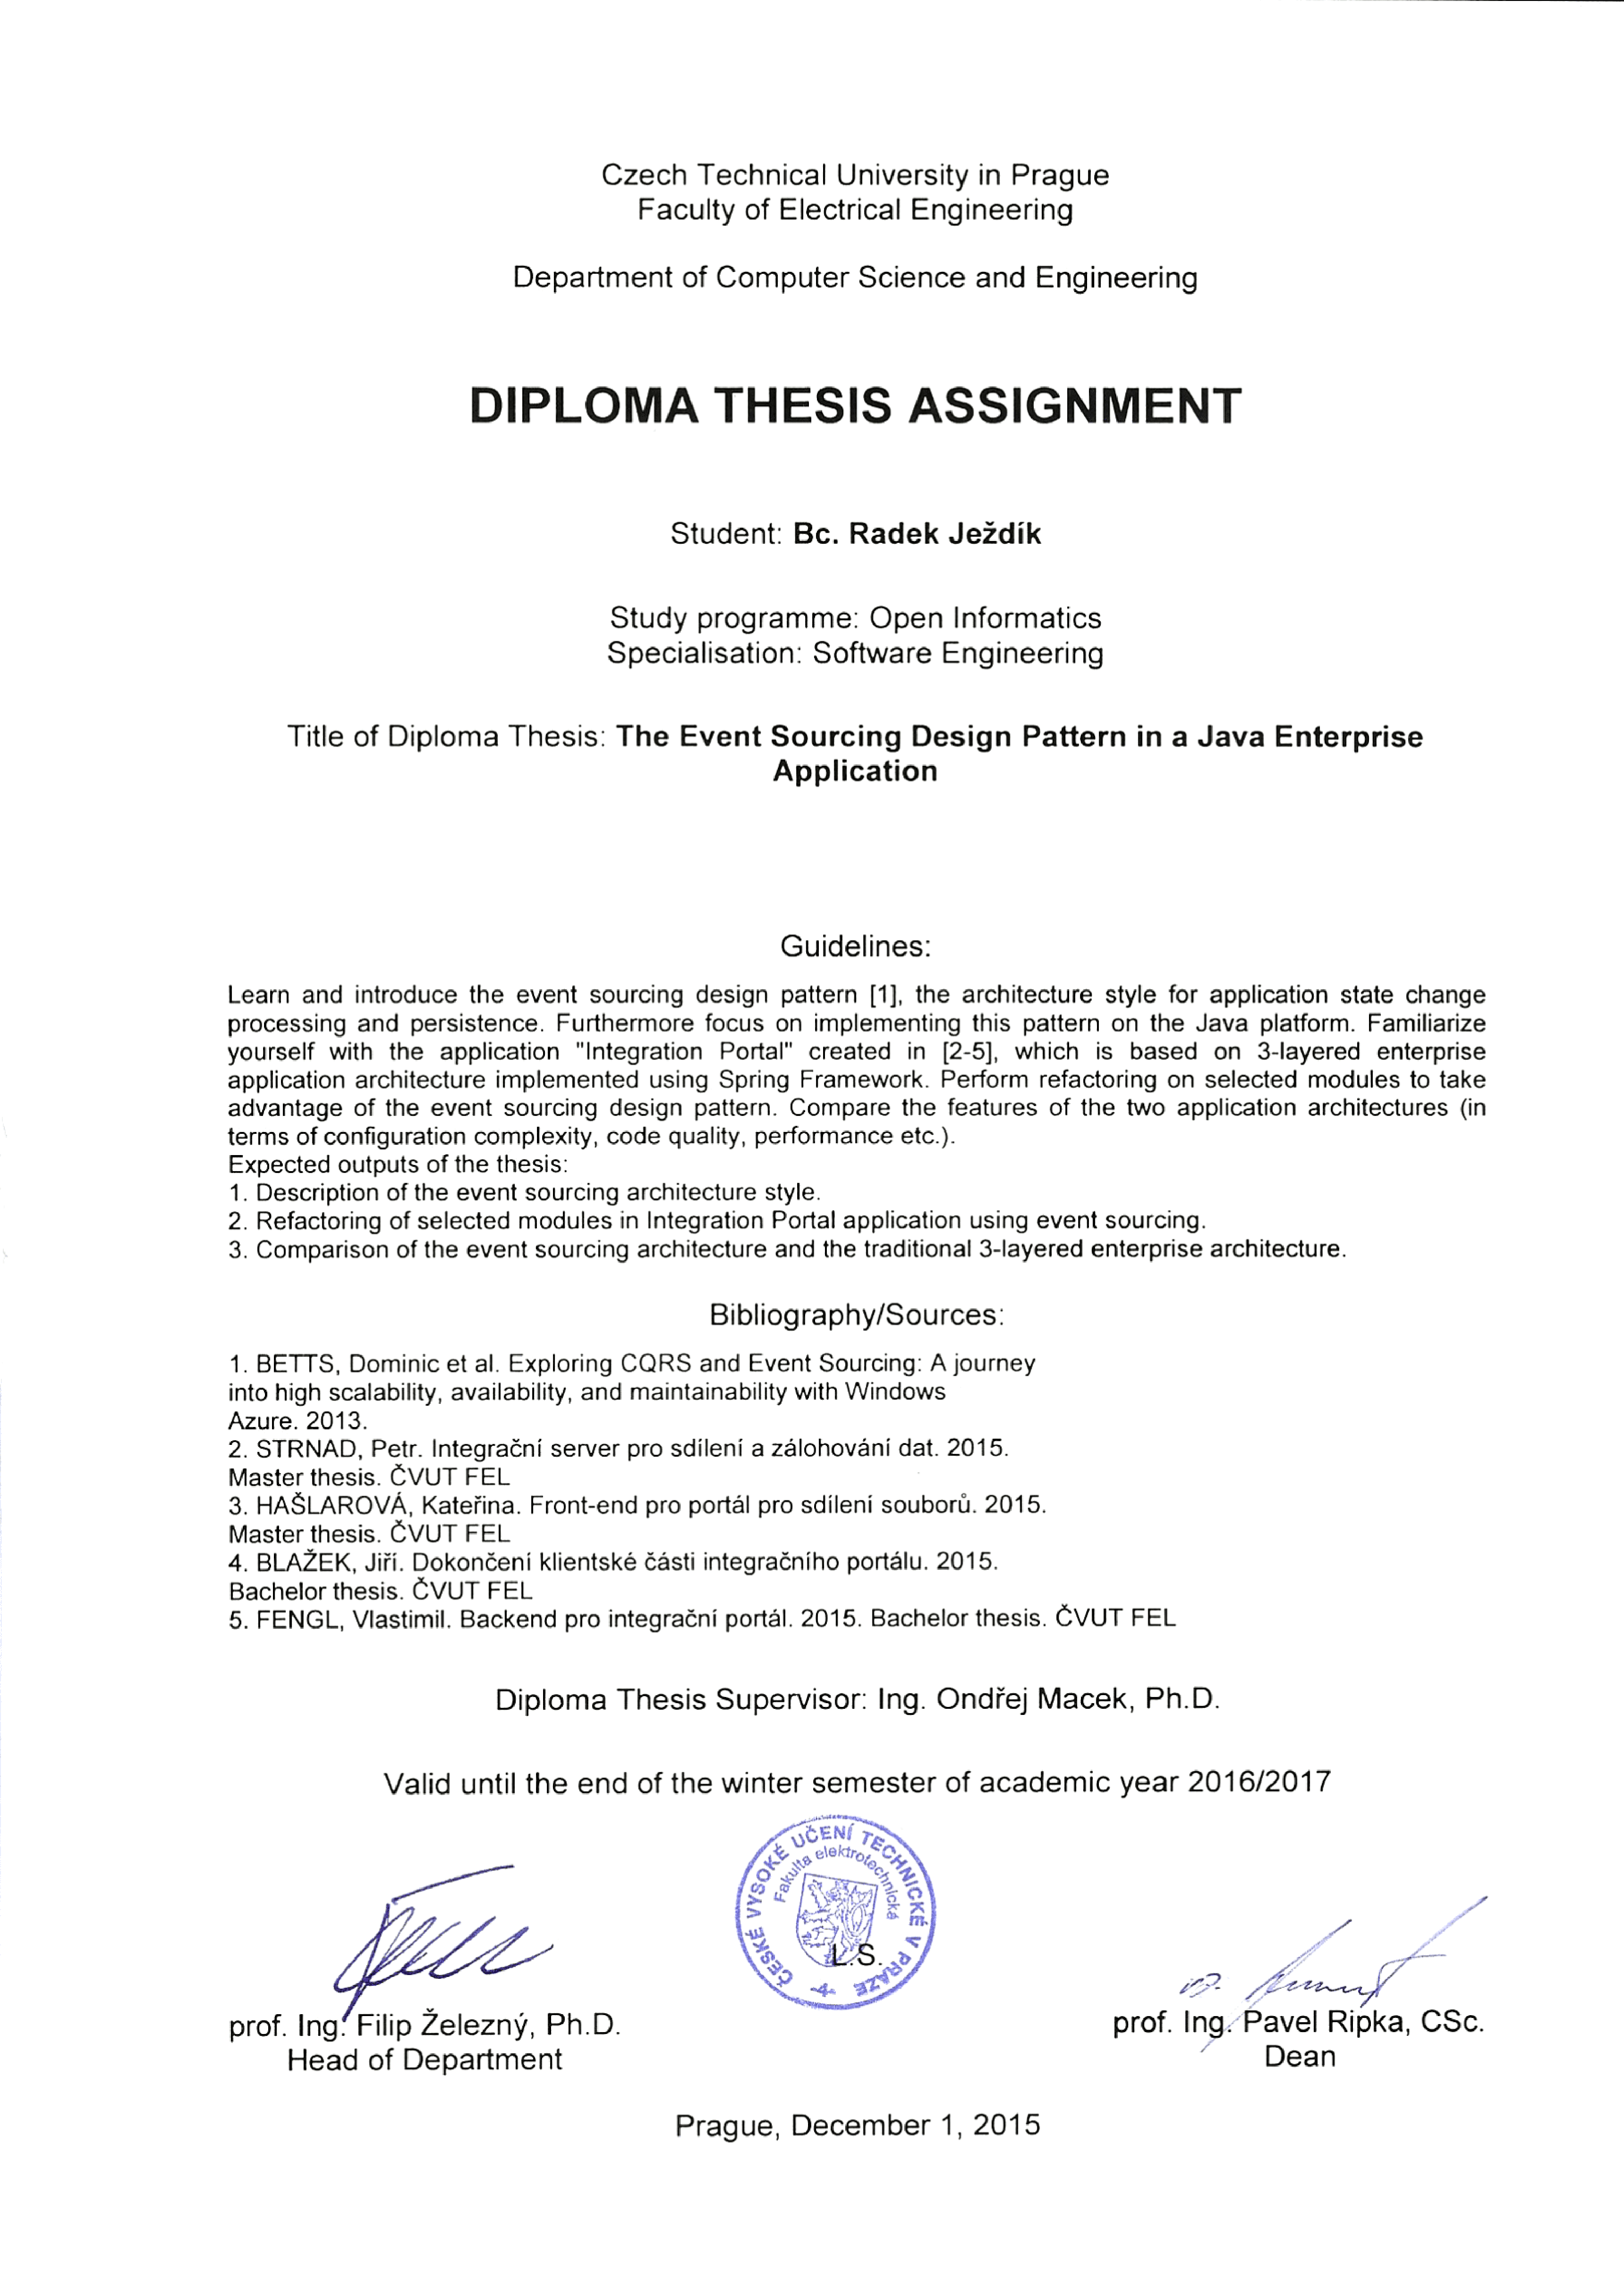
\includepdf{zadani.pdf}

	%%%%%%%%%%%%%%%%%%%%%%%%%%    
	% Titulni stranka / Title page 
	\coverpagestarts

	%%%%%%%%%%%%%%%%%%%%%%%%%%%    
	% Poděkovani / Acknowledgements 

	\acknowledgements
	\noindent
	**todo**
	Rád bych zde poděkoval své rodině, která mě po celou dobu studia podporovala. Dále bych chtěl poděkovat Ing. Ondřeji Mackovi, vedoucímu této bakalářské práce, za~odlehčený přístup a~komunikaci v~přátelském duchu.


	%%%%%%%%%%%%%%%%%%%%%%%%%%%   
	% Prohlášení / Declaration 

	\declaration{Prague, 5th of January\, 2015}


	%%%%%%%%%%%%%%%%%%%%%%%%%%%%    
	% Abstrakt / Abstract 
 
	\abstractpage

	**todo**This diploma thesis provides general information about the Event Sourcing design pattern and principles of closely associated CQRS (Command Query Responsibility Segregation) design pattern and their usage in the Java programming language. The aim of this thesis was to study these design patterns and apply them to a real-world software project. And finally, describe the advantages and disadvantages of this design over the traditional architecture found in most enterprise Java projects.

	% Prace v~cestine musi krome abstraktu v~anglictine obsahovat i
	% abstrakt v~cestine.
	%\vglue60mm

	%\noindent{\Huge \textbf{Abstrakt}}
	%\vskip 2.75\baselineskip

	%\noindent
	%Předmětem této práce je návrh a~vývoj webového nástroje pro tvorbu a~sdílení HTML prezentací. Cílem je vytvořit webovou aplikaci, která umožní tvorbu webových prezentací za~účelem jejich prohlížení a~sdílení. Obsahem této práce je analýza, návrh, imple\-mentace a~testování systému.

	%%%%%%%%%%%%%%%%%%%%%%%%%%    
	% obsahy a~seznamy
	\tableofcontents		% Obsah / Table of Contents 

	% pokud v~práci nejsou obrázky nebo tabulky - odstraňte jejich seznam
	\listoffigures			% Obsah / Table of Contents 
	% \listoftables			% Seznam tabulek / List of Tables

	%%%%%%%%%%%%%%%%%%%%%%%%%% 
	% začátek textu  
	\mainbodystarts




%%% DOC_CONTENT %%%




\bibliographystyle{csplainnat}
{
\def\CS{$\cal C\kern-0.1667em\lower.5ex\hbox{$\cal S$}\kern-0.075em $}
\bibliography{BP-ref}
}




%%%%%%%%%%%%%%%%%%%%%%%%%% 
% vše co následuje bude uvedeno v~přílohách
\appendix	

\printnomenclature

\chapter{Code listings}\label{chap:ukazkykodu}


\begin{lstlisting}[caption={Ukázka integračních testů},label={lst:integrationtest},
language=java,
numbers=left,
breaklines=true]
xxx
\end{lstlisting}

\newpage

\begin{lstlisting}[caption={Ukázka integračních testů},label={lst:integrationtest},
language=java,
numbers=left,
breaklines=true]
xxx
\end{lstlisting}


\chapter{XXX}\label{chap:loadtest}


\chapter{Contents of CD attachment}

\dirtree{%
.1 src/\DTcomment{zdrojové soubory aplikace}.
.1 text/.
.2 src/\DTcomment{zdrojové soubory dokumentu}.
.2 jezdirad-thesis-2013.pdf\DTcomment{elektronická verze dokumentu ve formátu PDF}.
.1 instalacni\textunderscore{}manual.pdf\DTcomment{návod na instalaci aplikace}.
.1 readme.txt\DTcomment{obsah CD a důležité informace}.
}



\end{document}

















